\chapter{Experimental Design}
\label{ch:experiments}
    % One planner, two environments
    The same planner runs in two environments.
    A synthetic harness generates planning problems at scale and is where the correctness and structural measurements are taken, and a simulated robot on ROS~2 is where the planner drives real motion (Section~\ref{sec:sim_harness}).
    The planner is the same code in both, so what the simulation exercises is the construction itself rather than a separate implementation of it.

\section{Problem Generation}
\label{sec:problem_generator}
    % What are the main parts of a problem?
    As defined by \probone and \probprime, a problem consists of a pool of interconnected states, an action database describing the transitions between them, an initial state, and a goal for the tree to regress from.
    Problems come from two sources.
    A randomized generator samples all four components, which supplies the volume needed for the structural comparisons.
    The layered domain fixes the transition structure allowing interference to be excluded from construction altogether.

    \subsection{Goal Shapes}
    \label{subsec:goal_shapes}
    % What are the types of goal structures?
    Both constructions accept goals beyond the AND-only case, so two goal shapes are used across the experiments.

    \input{figures/goal_shapes}

    A nested goal is a disjunction whose disjuncts share a conjunct, written with that conjunct factored out of the disjunction.
    It is the smallest shape in which the two constructions can differ, since the factored conjunct is what one construction expands once and the other duplicates.

    A deep goal adds a second disjunction alongside the first, so a DNF compilation enumerates four sub-goals rather than two when each disjunction is binary.

    A flat goal, in which the shared conjunct is written into every disjunct rather than factored out, is used only to check the equivalence of Section~\ref{sec:equivalence} (Section~\ref{subsec:pruning_comparison}).

    \subsection{Randomly Generating Problems}
    \label{subsec:random_generator}

    \input{figures/base_random_generator}
    
    % What does the random generator give us?
    The generator is inherited from the test setup of \cite{cai2021} and is parameterized by literals, distance, and iterations.
    A random initial state is first sampled from the literal set.
    The size of a state, and of the preconditions, additions, and deletions of an action, scale with the number of literals in the problem.
    From the initial state, preconditions, additions, and deletions are sampled to produce an action together with the state that action reaches.
    Repeating this step distance times yields a single path from the initial state to a final state.
    To diversify the pool, states are then drawn at random from it and new actions are created from them, producing branches that do not lie on the direct path to the final state.
    This step is repeated iterations times, and the states created during it join the pool.
    Since every pooled state is later scored for membership, these branches test whether a tree reaches the goal from states off the route the generator built.

    \subsubsection{Selecting Disjuncts}
    \label{subsubsec:disjunct_selection}
    % Review what disjuncts are
    A disjunct is an operand of a disjunction, so a goal with a single \pred{OR} offers the tree a choice between two disjuncts.
    Disjuncts are drawn from the states along the generated path rather than constructed independently of it, so every disjunct is satisfiable in at least one reachable state.

    % How each goal shape is drawn
    A nested goal is drawn from two distinct path states.
    A random subset of each is taken, the literals the two subsets share become the shared conjunct, and the remainders become the operands of the disjunction.
    A deep goal is drawn from two distinct path states in the same way, except that the shared conjunct is a random subset of the literals both states hold.
    The remainder of each subset is then split in half, giving one operand to each of the two disjunctions.
    A draw is discarded when the shared conjunct or any operand is empty, since the goal would then lack the structure its shape requires.

    % Subsumption
    A draw is also rejected when one operand of a disjunction contains the other.
    The disjunction is then equivalent to the smaller operand alone and offers no genuine alternative, so the goal would reduce to a simpler shape.

    % Why the initial state is not checked
    No draw is rejected for holding in the initial state, since the initial state plays no role in a fixpoint tree or its measurement (Section~\ref{sec:fixpoint}).

    Selection is attempted a limited number of times, and a pool that yields no admissible goal is discarded along with the problem built from it.

    \subsubsection{Admissibility and Reproducibility}
    \label{subsubsec:reproducibility}
    % When problems are rejected
    A problem is rejected when one of its disjuncts is satisfiable in no reachable state.
    This is tested using only the action database and no tree.
    A forward search runs from every state in the pool at once, applying every action whose preconditions hold until no new state is reached, and a disjunct counts as solvable if its literals are a subset of any state the search reaches.
    The rule matters most for a deep goal, whose disjuncts are combinations of two operands with nothing guaranteeing that a given combination is jointly reachable, so a goal may be disjunctive in form while offering only one viable route.
    Retaining it would report a construction as preserving every reachable state while one of its branches was never viable.

    Generation is not guaranteed to succeed on a given attempt.
    The randomized generator may produce a pool from which no admissible goal can be factored, in which case the attempt is discarded and another is made.
    Problems are drawn until a target count of admissible problems is reached rather than by making a fixed number of attempts, so the reported sample size is the number of problems measured.

    % Are random generator problems reproducable?
    Every run draws from a single seed fixed for the experiment, so reported results are reproducible from the seed and the configuration (Section~\ref{sec:configuration}) alone.

    \subsection{The Layered Domain}
    \label{subsec:layered_domain}
    % What the second source is for
    The second source of problems fixes the structure of a problem rather than sampling it, so that the effect of goal structure on the two constructions can be isolated from everything else.
    It is built from two disjoint pools of literals with no literals in common.

    \input{figures/layered_domain_setup}

    The first pool is a single linear chain of depth $d$, where each action advances one step along the chain and deletes its predecessor.
    The literal at the end of this chain is the shared conjunct of the goal.
    The second pool is $k$ linear chains of depth $m$, each beginning at a common start literal and advancing the same way, and the literal at the end of each is one disjunct of the goal.
    The goal is therefore $\pred{AND}(x_d, \pred{OR}(y^0_m, \ldots, y^{k-1}_m))$, and its disjunctive normal form is the $k$ conjunctions $\{x_d, y^b_m\}$.

    % Why this structure
    This structure places the duplication the two constructions differ over on an axis that can be varied directly.
    DNF compilation regresses each conjunction jointly, so the whole chain of the first pool is rebuilt inside every disjunct tree, while the unified construction expands it once.
    Varying $d$, $m$, and $k$ independently therefore moves the size difference between the two constructions without changing anything else about the problem.
    No action deletes a literal outside its own pool, so sibling subtrees cannot interfere, every arm is sound by construction, and the protect guard of Section~\ref{sec:interference} is inert.
    Interference is excluded by construction rather than measured, which separates the size measurement from the soundness question.
    The domain uses no randomness, so the action database, goal, initial state, and pool are determined by $d$, $m$, and $k$ alone, and a single run per configuration suffices.

    \subsubsection{Enumerating the States}
    \label{subsubsec:enumerating_states}
    % How the state pool is obtained
    The randomized generator produces its pool as a by-product of construction, since every state it samples or reaches while building actions joins the pool.
    The layered domain samples nothing, so its pool must be computed instead.
    Enumerating every subset of the literals is the only alternative that needs no starting point, and it is not a useful one.
    Almost every subset is unreachable, since a state holding two literals from the same chain describes a configuration the actions can never produce.

    The pool is therefore obtained by breadth-first search from $\{x_0, y_{\text{start}}\}$, the foot of both pools, applying every action whose preconditions hold and collecting the states reached.
    Because each chain step deletes its predecessor, the literals within a pool are mutually exclusive, so every reachable state holds exactly one literal from the first chain and one from the second.
    The search therefore terminates at $(d + 1)(1 + km)$ states, against $2^{(d+1)+(1+km)}$ subsets of the literal set.

\section{Planner Implementation}
\label{sec:planner_implementation}
    % Intro to section
    This section records the representation choices the planner rests on, built on the behavior tree semantics of Section~\ref{sec:background_bt}.

    % The blackboard / world state
    % TODO: Make sure the blackboard and how it serves as communication between nodes is in the background
    The world state is the set of literals currently true while the tree runs, and is the runtime counterpart of a state $s$ of Section~\ref{sec:problem_formulation}.
    It is held on the blackboard under a single registered key.
    Actions write to that key and conditions read from it, and no node holds a reference to any other, so the blackboard is the only channel through which a change made by one node becomes visible to another.

    % Conditions
    % TODO: Make sure to discuess what a behavior and what it returns is in py_trees in the background
    A condition is a behavior subclass holding a frozen set of literals and a protect set.
    When the node is ticked, it returns SUCCESS if its literals are a subset of the world state and FAILURE otherwise, which realizes the test $c \subseteq s$ of Section~\ref{sec:problem_formulation}.

    % Actions and the action factory
    An action is a behavior subclass holding precondition, add, and delete literal sets.
    When expansion selects an action, it does not instantiate the action node itself.
    It receives a function that builds the node from the action's name and the action database, so the planner carries no dependency on any particular action implementation.
    That function is the only seam between the planner and the environment it acts in, and it is what allows the synthetic and simulated settings to share one builder.

    % Traversals
    Traversals are implemented behind a common interface that takes the root of the tree together with the record of expanded conditions and returns the next condition to expand, or nothing once none remains.
    The builder is parameterized by a traversal rather than containing one, so changing the order in which conditions are selected requires no change to the builder.
    Each traversal policy a experiment uses is described in Section~\ref{subsec:settings}.
    
    % Goal Structure Nodes
    \texttt{GoalSequence} and \texttt{GoalSelector} subclass the \texttt{py\_trees} sequence and selector without overriding anything, so they tick exactly as their parent classes do.
    They exist so that the traversal and scoping routines can recognize goal structure by node type rather than by inspecting children.

    % Keys and root replacement    
    The expansion record is keyed on a condition's literals and protect set rather than on node objects, and each key maps to the set of branch scopes in which it has been expanded.
    Two structurally identical conditions therefore share a key, and a condition is eligible for expansion only if its scope is not yet in that key's set.
    
    % Feature flags
    Protection mode, pruning scope, and subset pruning are set per experiment (Section~\ref{sec:configuration}).
    
\section{Building Fixpoint Trees}
\label{sec:fixpoint}
    % Why expansion must run to a fixed point
    A direct comparison between tree architectures requires that both be expanded to the same degree.
    For these experiments every tree, DNF or unified, is expanded completely.
    A tree is at its fixpoint when every condition in it has been expanded within its branch scope, so that a further expansion step would leave the tree unchanged.
    A tree built by expanding until it reaches this point is called a fixpoint tree.
    Full expansion needs no initial state, since the fixpoint is a property of the tree and the action database alone.
    A fixpoint tree therefore does not depend on where the robot starts.
    
    This is what makes a direct region of attraction measurement possible.
    Only one tree is built per problem, and every state in the pool is scored against it to determine whether that state lies within the tree's region of attraction, Section~\ref{sec:membership}.
    In contrast, the expansion loop of \cite{cai2021} stops once the tree can act from $s_0$.
    That yields a tree determined by the initial state, and scoring a pool against it would measure the starting state as much as the construction.

    \input{figures/fixpoint_tree}

    % The fixpoint loop
    Building a fixpoint tree begins with the base tree structured from the goal, carrying the \texttt{GoalSequence} and \texttt{GoalSelector} nodes the goal calls for.
    An unexpanded condition is then selected, expanded following the expansion step of \cite{cai2021}, and recorded.
    The scoped pruning of Section~\ref{sec:pruning} is then applied.
    The process repeats until no unexpanded condition remains.

    % What unexpanded means
    % TODO: Make sure prop 4 in background
    The loop terminates because the keys and scopes of the expanded record (Section~\ref{sec:planner_implementation}) are both drawn from finite sets.
    Distinct condition sets are bounded as in Proposition~4 of \cite{cai2021}, and the branch scopes are bounded by the goal structure.
    Expansion order does not affect the resulting tree, as established in Section~\ref{subsec:order_independence}.

    % Why is fixpoint used on DNF and Unified
    The unified arm calls the fixpoint builder once on the composed goal.
    The DNF arm calls the same builder once per disjunct and joins the results under a fallback.
    Both arms therefore share an action model, an expansion step, and a termination condition, offering the only difference between them to be the goal structure each was built from.

    A tree expanded online stops growing once it has a route that runs from the current state, so it can be smaller and cover fewer states than the fixpoint tree for the same goal, as the simulation run of Section~\ref{sec:results_sim} shows.
    
\section{Measuring Region of Attraction}
\label{sec:membership}
    % What does membership mean? Restate problem 1` in terms of membership
    The region of attraction $R_g$ of Section~\ref{sec:problem_formulation} is measured by ticking the tree from every state of a pool and testing the goal against the resulting world state, independently of the root's status.

    \subsection{Membership Guards}
    \label{subsec:membership_guards}
    % What guards does the membership test have
    Before any candidate is tested, every composite in the tree is checked for memory and the run is rejected if any carries it, since the analysis of Section~\ref{sec:interference} assumes composites that re-tick every child on every tick, and a composite with memory would hide sibling interference.
    
    The actions of the synthetic problems complete within the tick that runs them and never report RUNNING, so the root returns only SUCCESS or FAILURE.
    This is asserted on every tick, so an action that failed to complete within its tick would halt the run rather than be silently classified.

    \subsection{Membership Test Procedure}
    \label{subsec:membership_procedure}
    % The procedure of the membership test
    Each state tested for membership is referred to as a candidate state.
    Because actions add and remove literals as they run, each candidate is copied before it is handed to the tree, so the pool is not altered by testing against it.
    Every node is then returned to an INVALID status, which assures that no status survives from a previously tested candidate.

    The tree is ticked, and the goal is evaluated against the resulting world state by descending its \pred{AND}/\pred{OR} structure, independently of any node's status.
    The world state changes only when an action writes to the blackboard, so the resulting state is also compared with the state before the tick, and a tick that leaves it unchanged is called stationary.
    Since composites carry no memory and every action completes within its tick, the outcome of a tick is determined by the world state it starts from, so a stationary tick would repeat on every later tick and the run can be classified at that point.
    Otherwise ticking repeats, up to a fixed budget that realizes the finite time requirement of \probprime.

    \subsection{Membership Results}
    \label{subsec:membership_outcomes}
    % The 5 outcomes of the test
    Each candidate falls into one of five outcomes.
    A candidate is a member of $R_g$ when the root returns SUCCESS and the goal holds in the resulting world state.
    The remaining four outcomes are ways a candidate fails to be a member, and they differ in why it fails.

    An honest failure occurs when a tick is stationary and the root reports FAILURE.
    A violation occurs when a tick is stationary and the root reports SUCCESS on an unsatisfied goal, so the tree will report SUCCESS on every later tick without the goal holding.
    A cycle occurs when a tick changes the world state into one already seen earlier in the run, so the tree keeps acting but has entered a loop and will not terminate.
    A cap occurs when the tick budget is exhausted without the run resolving into any of the other outcomes, and since a capped state is counted outside $R_g$, a reported region is a lower bound on the true one.
    
    % False successes
    A false success is counted per tick rather than per candidate.
    It is a tick on which the root reports SUCCESS while the goal does not hold in the resulting state.
    If the tick is not stationary, ticking continues and the candidate may still become a member, so a member can accumulate false successes, and only a stationary false success makes the candidate a violation.

    \subsection{Preservation}
    \label{sec:membership_set_comparison}
    % What is preservation?
    Each arm is compared with the DNF reference state by state rather than by coverage alone, since two arms covering the same number of states may cover different ones.
    The fraction of the reference's members that an arm also covers is its preservation.
    States the arm covers and the reference does not are counted separately, so an arm that trades coverage can be told apart from one that only loses it.
    
    Figures over a sample of problems are reported with 95\% bootstrap intervals, computed by drawing the problem set again with replacement 2000 times, recomputing the figure on each draw, and taking the middle 95\% of the results.
    Whole problems are resampled rather than individual states, since the states of one problem share an action database and goal and are not independent.

    \subsection{Pools and Reachability}
    \label{sec:membership_pools_reachability}
    % Where does the denominator of the ROA come from
    Running the membership test across a pool yields the subset of pooled states that lie in $R_g$.
    Where a single figure is reported rather than a set comparison, that subset is expressed as a fraction, and two denominators are used.

    % The pool
    The first is the pool itself.
    The pool of the layered domain is the complete reachable set, computed by breadth-first search from the initial state (Section~\ref{subsubsec:enumerating_states}).
    The pool of the randomized generator is sampled during generation, so a fraction of it describes the sampled states.

    % The solvable states
    A pooled state may admit no plan to the goal under any tree, and no construction can be expected to cover it.
    The second denominator therefore counts only the solvable states, the pooled states from which some sequence of actions reaches $S_g$.
    Each is identified by an exhaustive forward search from the state over the action database, independently of any tree, and the search terminates because the state space is finite.
    A state from which a tree reaches the goal must be solvable, so a member outside this set would indicate a defect in the harness, and the soundness sweep halts if one occurs.

    % What each denominator is used for
    The share of solvable states a tree covers measures its completeness on the pool, independently of any other construction.
    Chapter~\ref{ch:results} reports the share of pooled states where every outcome of the membership test is shown, and the share of solvable states where completeness is the question.

\section{Simulation Harness}
\label{sec:sim_harness}
    % Scope of the ROS development
    The simulation harness runs the planner on a simulated robot with a navigation stack.
    It provides three things the synthetic harness cannot, namely actions that occupy time across many ticks, and  literals derived from perception rather than written by actions.
    It is a demonstration rather than an evaluation, so it tests no proposition and reports no quantity.

    \subsection{The Simulated World}
    \label{subsec:sim_world}
    % The simulated world
    The simulated world runs in Gazebo and contains three rooms, shown in Figure~\ref{fig:sim_world}.
    Room~B is a hub that spans the right side of the building, and rooms~A and~C are reached from it through one door each.
    Each room is described by a goal pose for navigation and a rectangle used to classify the robot's pose into that room (Section~\ref{subsec:sim_perception_literals}).
    The robot spawns at the hub's goal pose.

    \begin{figure}[htbp]
        \centering
        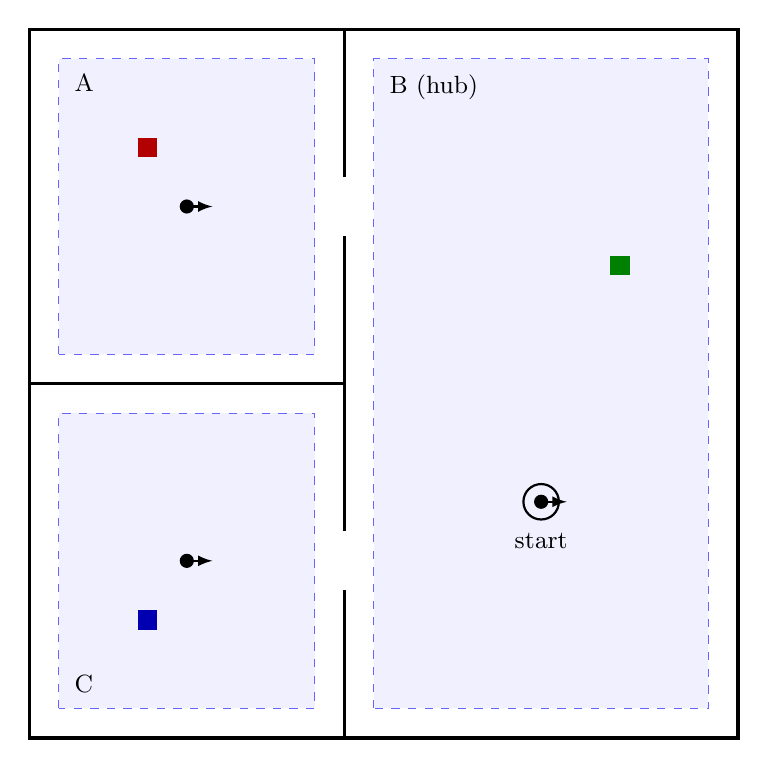
\begin{tikzpicture}[x=0.5cm, y=0.5cm, font=\small]
            % Room rectangles used by the pose observer
            \fill[blue!6]  (-3.25, 0.75) rectangle (3.25, 8.25);
            \fill[blue!6]  (4.75, -8.25) rectangle (13.25, 8.25);
            \fill[blue!6]  (-3.25, -8.25) rectangle (3.25, -0.75);
            \draw[blue!60, dashed] (-3.25, 0.75) rectangle (3.25, 8.25);
            \draw[blue!60, dashed] (4.75, -8.25) rectangle (13.25, 8.25);
            \draw[blue!60, dashed] (-3.25, -8.25) rectangle (3.25, -0.75);

            % Walls
            \draw[line width=1.2pt] (-4, -9) rectangle (14, 9);
            \draw[line width=1.2pt] (-4, 0) -- (4, 0);
            \draw[line width=1.2pt] (4, -9) -- (4, -5.25);
            \draw[line width=1.2pt] (4, -3.75) -- (4, 3.75);
            \draw[line width=1.2pt] (4, 5.25) -- (4, 9);

            % Obstacles
            \fill[red!70!black]   (-1.25, 5.75) rectangle (-0.75, 6.25);
            \fill[blue!70!black]  (-1.25, -6.25) rectangle (-0.75, -5.75);
            \fill[green!50!black] (10.75, 2.75) rectangle (11.25, 3.25);

            % Goal poses, facing +x
            \foreach \x/\y in {0/4.5, 9/-3, 0/-4.5} {
                \draw[-latex, thick] (\x, \y) -- (\x + 0.65, \y);
                \fill (\x, \y) circle (0.18);
            }

            % Start pose, at the hub's goal pose
            \draw[thick] (9, -3) circle (0.45);
            \node[anchor=north] at (9, -3.55) {start};

            % Labels, inside each room's rectangle
            \node[anchor=north west] at (-3.1, 8.1) {A};
            \node[anchor=north west] at (4.9, 8.1) {B (hub)};
            \node[anchor=south west] at (-3.1, -8.1) {C};
        \end{tikzpicture}
        \caption[Simulation world]{The simulation world. Thick lines are walls, with a door between the hub and each side room. Shaded rectangles with dashed borders are the regions the pose observer uses to classify the robot into a room. Dots with arrows are the navigation goal poses of the three rooms, and the open circle marks the start pose, which coincides with the hub's goal pose. Small squares are static obstacles.}
        \label{fig:sim_world}
    \end{figure}

    \subsection{ROS Trees}
    \label{subsec:sim_ros_trees}
    % TODO: define a disturbance in background
    % How the tree is implemented in ROS
    The simulated tree is built with \texttt{py\_trees\_ros}, which adapts \texttt{py\_trees} to behavior trees running inside ROS~2 nodes.
    Each iteration of the runner services ROS callbacks and then ticks the tree, so the blackboard reflects the most recent perception before the tree acts on it.
    The runner loops without terminating, so a disturbance arriving at any point is acted on, including after the goal has been reached.

    % Interleaved expansion
    The tree starts as the base tree of the goal and grows while it runs.
    On a tick that ends in RUNNING the runner lets the running action continue.
    On a tick that ends in FAILURE, the runner expands one condition before the next tick.
    Expansion and execution therefore interleave on the same tree.
    The runner also evaluates the goal against the world state on every tick, independently of the tree, and counts a false success whenever the root reports SUCCESS while the goal does not hold.

    \subsection{Literals from Perception}
    \label{subsec:sim_perception_literals}
    % Literal states come from perception
    The room literals are maintained by a background \texttt{PoseObserver} node rather than by the actions.
    The observer classifies the localized pose into the room whose rectangle contains it.
    The rectangles are inset from the walls, so a pose in a doorway falls in no rectangle and leaves the last room literal in place.
    The gap between rectangles therefore acts as hysteresis, and a pose near a boundary does not alternate between rooms.
    Every other literal is written by the action that adds or deletes it, in the same update in which that action returns SUCCESS, as in the synthetic harness.

    % Inversion and early effects
    For the room literals this inverts the arrangement of the synthetic harness, where the action that moves the robot also writes the literal.
    Here an action triggers motion and a separate observer reports what resulted, so the tree acts on what perception reports rather than on what the action intended.
    Because the observer runs independently of the tree, it can write a room literal while a move toward that room is still running, as soon as the robot enters the room's rectangle.
    Such an update reaches the tree between ticks, like any other change to the world state.

    \subsection{Nav2 Actions}
    \label{subsec:sim_nav2_actions}
    % Actions with Nav2
    Every action is carried out by a Nav2 server.
    A move action sends a NavigateToPose goal for the target room's goal pose, and actions without travel use the Spin and Wait behavior servers.
    While its server is working the action returns RUNNING, so it remains running across many ticks rather than resolving within the tick that started it.

    % Gating on the observed literal
    Proposition~\ref{prop:left_soundness} assumes that an action's effects hold once it returns SUCCESS.
    Actions that write their own literals meet this by construction.
    A move action does not write its room literal, so it returns SUCCESS only once Nav2 reports the goal pose reached and the observer has written the target room literal.
    Without that gate it could report SUCCESS on Nav2's result before its effect was in the world state.

    % Halting and early effects
    An action stops being ticked once the condition above it holds.
    For a move this happens either when it succeeds or when the observer writes the target literal early (Section~\ref{subsec:sim_perception_literals}).
    In the second case the tree halts the move on the next tick, which cancels its navigation goal.
    The early update arrives between ticks, and Proposition~\ref{prop:left_soundness} holds in every state the tree is ticked in, so an early effect cannot cause a false success.

    % What if the action fails?
    An action that fails during execution causes an expansion before the next tick, since the runner does not distinguish execution failure from the absence of an applicable action.

\section{Experiment Configuration}
\label{sec:configuration}
    % TODO Revise entire section once results is done
    % The point of this section
    Every figure reported in Chapter~\ref{ch:results} comes from a named configuration of the procedures described in this chapter.
    Three synthetic experiments are reported, the construction comparison, the soundness sweep, and a comparison of expansion scopes, together with the simulation demonstration.
    The three synthetic experiments share the planner implementation, the fixpoint construction, and the membership test, and differ only in the arms they compare and the settings listed here.

    \subsection{Reference Arm}
    \label{subsec:reference_arm}
    % Design of the reference DNF tree used in almost every test
    A DNF tree serves as the reference every other arm is scored against.
    Protection is off in the reference, which is faithful rather than an oversight, since the construction being compared against has no such  mechanism.
    The omission is also harmless to it, as a DNF subtree carries a single conjunctive goal condition and therefore has no sibling goals to interfere with, which is the failure protection exists to prevent.
    
    % Whether the reference covers every solvable state
    Preservation measured against the reference equals coverage of the solvable states only if the reference itself covers every solvable state.
    That is not assumed.
    The solvable states of Section~\ref{sec:membership_pools_reachability} are computed independently of any tree, and Chapter~\ref{ch:results} reports how the region of the reference compares with them.

    % What the baseline arm leaves out
    The DNF arm implements the construction as published and nothing beyond it.
    Two refinements of \cite{chen2024} are absent.
    Compaction, which factors common literals out of adjacent conditions, is omitted because it is orthogonal to the comparison being made, as the same factoring could be applied to either construction.
    Cost-sorted assembly is omitted because the order of subtrees under the fallback changes neither the node set nor the success region of a fully expanded tree.
    The node ratio of an arm is the geometric mean over problems of the reference's node count divided by the arm's, so a value above one means the arm builds the smaller tree.
    Compaction would reduce the node count of the reference if applied, so the node ratios reported in Chapter~\ref{ch:results} are upper bounds on the size difference between the constructions rather than exact measurements of it.

    \subsection{Compactness Sweep}
    \label{subsec:construction_comparison}
    % What does this test cover?
    The compactness sweep measures the unified construction against DNF compilation as a function of goal structure, rather than over a sample of randomly generated problems.
    The unified arm is one tree built from the composed goal.
    The DNF arm is one fixpoint tree per disjunct, joined under a fallback so that the sweep has a single root to tick.

    Problems come from the layered domain of Section~\ref{subsec:layered_domain}.
    One parameter varies at a time while the other two hold at their base values, with chain depth $d$ taking twelve values, branch depth $m$ five, and branch count $k$ five.
    The base configuration appears in all three, giving twenty distinct configurations.

    Tree size is measured as the total node count of the fixpoint tree, the measure used by \cite{cai2021}.
    Condition counts, distinct condition counts, and expansion counts are recorded alongside it for both arms, together with the ratios between them.
    The membership buckets and false success counts are recorded as well, not as a result but as a check that the isolation held.
    % A difference in region of attraction between the two arms would indicate a defect rather than a finding.

    \subsection{Soundness and Preservation Sweep}
    \label{subsec:soundness_and_preservation_sweep}
    % What does this test cover?
    The soundness sweep measures the effect of the protection modes within the unified construction.
    Each unified arm is scored against a DNF reference built from the same problem.

    Four arms are compared, the unified construction with protection off, with protection against left siblings, with protection against all siblings, and the reference.
    The five membership outcomes of Section~\ref{subsec:membership_outcomes} are recorded for each arm, together with the false success count, the number of times protection rejected an action during construction, and the number of solvable states in the pool.

    Problems come from the randomized generator, so interference arises at whatever rate the sampler produces rather than being set.
    Nested and deep goals are run as separate samples of one thousand admissible problems each, admitted under the subsumption check of Section~\ref{subsubsec:disjunct_selection} alone.
    A flat goal places no \texttt{GoalSequence} in the tree, so it has no sibling goals to protect and every protection mode would produce the same tree.

    \subsection{Scoped and Global Expansion}
    \label{subsec:pruning_comparison}
    % What does this test cover?
    The scope comparison measures the scoped expansion record and pruning of Section~\ref{subsec:pruning_scopes} against the global rule of \cite{cai2021}.
    It reuses the problems of the soundness sweep, one thousand nested and one thousand deep goals, so its scoped arms are the unified arms of that sweep.
    Each problem is built again under the global rule, once with protection off and once against left siblings, and scored against the same DNF reference.
 
    The global arms are built by a parallel loop that shares one record of expanded conditions across branches and applies the unscoped pruning test.
    That loop also expands until no unexpanded condition remains, so the scoped and global arms are expanded to the same degree.
    Subset pruning is enabled in every arm.
    The membership outcomes and tree size are recorded for each arm, together with the states it solves that the reference does not and the reverse.
 
    Two further checks isolate the mechanisms of Section~\ref{sec:pruning}.
    The global arm under left protection is rebuilt with a record key that ignores the protect set, while protection still filters actions, which separates the effect of the key from the effect of the actions protection rejects.
    A flat goal is also built from each nested problem by writing the shared conjunct into both disjuncts, and its scoped tree is compared with the DNF reference in node count and region of attraction.

    \subsection{Simulation Demonstration}
    \label{subsec:sim_configuration}
    % What is configured for the demonstration
    The simulation demonstration runs once, on a single task, under the tick-driven loop of Section~\ref{subsec:sim_ros_trees} rather than to a fixed point, so its tree depends on the state the robot starts in.
    Its task and settings are given with the run in Section~\ref{subsec:sim_setup}.

    \subsection{Experiment Settings}
    \label{subsec:settings}
    % TODO: Scoped BFS define it
    \begin{table}[htbp]
        \centering
        \caption{Configuration of each experiment.}
        \label{tab:settings}
        \small
        \begin{tabular}{llll}
        \toprule
        & Soundness & Compactness & Scope \\
        \midrule
        \multicolumn{4}{l}{\emph{Problem}} \\
        Source              & Randomized           & Layered              & Randomized \\
        Goal shape          & Nested, deep         & Nested               & Flat, nested, deep \\
        Generator           & $10/10/10$           & ---                  & $10/10/10$ \\
        Admission checks    & Subsumption          & ---                  & Subsumption \\
        Swept               & ---                  & $d$, $m$, $k$        & --- \\
        Base values         & ---                  & $d{=}3$, $m{=}2$, $k{=}2$ & --- \\
        \midrule
        \multicolumn{4}{l}{\emph{Construction}} \\
        Arms                & Off, left,           & Unified, DNF         & Scoped and global, \\
                            & symmetric, DNF       &                      & each off and left \\
        Reference           & DNF                  & DNF                  & DNF \\
        Protection          & Off, left, symmetric & Off, inert           & Off, left \\
        Pruning             & Scoped               & Scoped               & Scoped, global \\
        Subset pruning      & Enabled              & Enabled              & Enabled \\
        Traversal           & Scoped BFS           & Scoped BFS           & Scoped BFS, BFS \\
        \midrule
        \multicolumn{4}{l}{\emph{Run}} \\
        Problems            & 1000 per shape       & 20 configurations    & 1000 per shape\\
        Tick cap            & 100                  & 100                  & 100 \\
        Seed                & 0                    & Deterministic        & 0 \\
        \bottomrule
        \end{tabular}
    \end{table}

    The randomized generator is configured with ten literals, a distance of ten, and ten branching iterations, which is the configuration of \cite{cai2021}.
    The soundness sweep and the scope comparison share their problems.